\documentclass[12pt]{article}

\usepackage[latin1]{inputenc}
\usepackage{amssymb}
\usepackage{amsmath}
\usepackage{amsthm}
\usepackage{latexsym} 
\usepackage{graphicx}
\usepackage{bm}  
\usepackage{overpic} 
\usepackage[normalem]{ulem}
\usepackage{enumitem}
\usepackage{subcaption}

  
\usepackage{exscale}
\usepackage{amsfonts}
\usepackage[usenames,dvipsnames]{color} % load color package

\textwidth=6.0in \textheight=8.8in \hoffset=-0.2in
\voffset=-0.85in
\parskip=6pt
\baselineskip=9pt
\topmargin 0.8in
 
\def\black#1{\textcolor{black}{#1}}
\def\blue#1{\textcolor{blue}{#1}}
\def\red#1{\textcolor{red}{#1}}
\def\green#1{\textcolor{green}{#1}}
\def\yellow#1{\textcolor{yellow}{#1}}
\def\orange{\textcolor{BurntOrange}}

\newtheorem{definition}{Definition}[section]
\newtheorem{lemma}{Lemma}[section]
\newtheorem{remark}{Remark}[section]
\newtheorem{example}{Example}[section]
\newtheorem{theorem}{Theorem}[section]
\newtheorem{cor}{Corollary}[section]
\newtheorem{corollary}{Corollary}[section]

\numberwithin{equation}{section}

\newcommand{\E}{\mathbb{E}}
\newcommand{\R}{\mathbb{R}}
\newcommand{\sigl}{\sigma_L}
\newcommand{\BS}{\rm BS}
\newcommand{\p}{\partial}
\newcommand{\var}{{\rm var}}
\newcommand{\cov}{{\rm cov}}
\newcommand{\beaa}{\begin{eqnarray*}}
\newcommand{\eeaa}{\end{eqnarray*}}
\newcommand{\bea}{\begin{eqnarray}}
\newcommand{\eea}{\end{eqnarray}}
\newcommand{\ben}{\begin{enumerate}}
\newcommand{\een}{\end{enumerate}}


\def\cC{\mathcal C}
\def\cD{\mathcal D}
\def\cS{\mathcal S}
\def\cH{\mathcal H}
\def\cI{\mathcal I}
\def\cJ{\mathcal J}
\def\cL{\mathcal L}
\def\cV{\mathcal V}
\def\cR{\mathcal R}
\def\bR{\mathbb R}
\def\cX{\mathcal X}
\def\cF{\mathcal F}
\def\bP{\mathbb P}
\def\bE{\mathbb E}
\def\bN{\mathbb N}
\def\bT{\mathbb T}
\def\bC{\mathbb C}
\def\var{\text{var\,}}
\def\eps{\varepsilon}

\newcommand{\mt}{\mathbf{t}}
\newcommand{\mS}{\mathbf{S}}
\newcommand{\tC}{\widetilde{C}}
\newcommand{\hC}{\widehat{C}}
\newcommand{\tH}{\widetilde{H}}
\renewcommand{\O}{\mathcal{O}}
\newcommand{\dt}{\Delta t}
\newcommand{\tr}{{\rm tr}}

\begin{document}



\title{{\bf{\Large{Early Exercise Premium in rBergomi Model}}}\\\vskip.5em \large{Within a Tree Framework}}


\author{ShengQuan Zhou\footnote{Department of Mathematics, Baruch College, CUNY. {\tt  szhou80@bloomberg.net}}{\setcounter{footnote}{1}} }

%\date{This version: December 25, 2011}


\maketitle\thispagestyle{empty}
 
%%***************************************************************************
%%
%%  Document begins here
%%
%%***************************************************************************



\begin{abstract}
In this report, we systematically examine the early exercise premium of American put options in rough Bergomi model as a function
of option moneyness, time to expiration, vol of vol, spot-vol correlation, and volatility roughness. The results are compared with a local volatility model calibrated to the vanilla smile generated by the rough Bergomi model. Both the rough Bergomi model and the local volatility model are implemented within a tree framework.
\end{abstract}

%%%%%%%%%%%%%%%%%%%%%%%%%%%%%%%%%%%%%%%%%%%%%%%%%%%%%%%%%%%%%%%%%%%%%%%%%%%%%%%%%
%
%
%  Section: Introduction
%
%
%%%%%%%%%%%%%%%%%%%%%%%%%%%%%%%%%%%%%%%%%%%%%%%%%%%%%%%%%%%%%%%%%%%%%%%%%%%%%%%%%%

\section{Introduction}
The empirical foundation of rough volatility lies in the remarkable consistency, for any reasonable timescale $\Delta$ of practical interest, between the time series of realized variance and the simple model \cite{gatheral1}
\begin{align}
\label{empiricaltimeseries}
\log \sigma_{t+\Delta} - \log\sigma_t = \nu (W_{t+\Delta}^H - W_t^H),
\end{align}
where $W^H$ is a fractional Brownian motion with Hurst exponent $H<\frac{1}{2}$ and $\nu>0$ is interpreted as the vol of vol. Recently, rough volatility is gaining popularity as a pricing model. In a simple case, the rBergomi model is a parsimonious model that fits the SPX volatility smile and explains the power-law behavior of the term structure of ATM volatility skew 
\begin{align}
\label{skewtermstructure}
\psi(\tau) \triangleq \Big| \frac{\partial}{\partial k}\sigma(k,\tau) \Big|_{k=0} \sim \frac{1}{\tau^{1/2-H}}
\end{align}
for small $\tau$, where $\tau$ is the time to expiration and $k=\log \frac{K}{S}$ is the logarithmic moneyness. The Hurst exponent extracted from the time series of realized variance Eq.(\ref{empiricaltimeseries}) is called \textit{realized roughness}. If one really believes in rough volatility model, the power-law exponent of the term structure of ATM volatility skew in Eq.(\ref{skewtermstructure}) can be interpreted as \textit{implied roughness}. 

\subsection{Prior Literature on Rough Volatility}
The empirical foundations of rough volatility were first established in Gatheral, Jaisson, and Rosenbaum \cite{gatheral1}. The initial path to pricing under rough volatility is set by Bayer, Friz, and Gatheral \cite{bayer}. Pricing VIX futures and options under rough volatility is further investigated by Jacquier, Martini, and Muguruza \cite{jacquier1}. Efficient simulation algorithms are discussed in detail by Horvath, Jacquier, and Muguruza \cite{horvath}. A joint calibration of rBergomi model to SPX volatility and VIX volatility has seen only limited success \cite{bayer}.

\subsection{Goal and Method of This Work}
This work sets out to calculate the early exercise premium associated with American options under rough volatility (rBergomi in this report) and examine its dependence on the model parameters. To benchmark the results, the early exercise premium is compared with a local volatility model calibrated to the volatility smile generated by the rBergomi model. Absence of Markovianity rules out any finite-dimensional PDE-based schemes and Monte Carlo simulations does not handle early exercise easily. Tree-based methods is the only approach. In this report, we implement the rBergomi model using a non-recombining quadrinomial (hence bushy) tree \cite{horvath}. To be consistent in style, the benchmarking local volatility model is implemented using the binomial implied volatility tree of Derman and Kani \cite{derman}.

\section{Specification of rBergomi Model}
\label{rbergomitree}
The price process in the rough Bergomi (rBergomi) model may be written in terms of the logarithmic price process: $X_t \triangleq \log S_t$: 
\begin{align}
\label{spec21} dX_t &= -\frac{1}{2}V_t dt + \sqrt{V_t}dB_t, \quad X_0 = 0\\
\label{spec22} V_t &= \xi_0(t)\exp\left( 2\nu C_H \mathcal{V}_t - \frac{\nu^2 C_H^2 t^{2H}}{H} \right), \quad V_0 > 0,
\end{align}
%We choose, among other integral representations of fractional Brownian motion, $W_t^H = C_H \mathcal{V}_t$, 
where $C_H \triangleq \sqrt{\frac{2H\times\Gamma(3/2-H)}{\Gamma(1/2+H)\times\Gamma(2-2H)}}$ and
%where
\begin{align}
\label{spec12}
\mathcal{V}_t \triangleq \int_0^t (t-u)^{H-1/2} dW_t.
\end{align}
The standard Brownian motion $Z_t$ driving the price and the 
%fractional Brownian motion $W_t^H$ 
Riemann-Liouville process $\mathcal{V}_t$ driving the volatility are correlated in the sense that $\mathbb{E}[dZ_t dW_t] = \rho dt$. \underline{Note}: whether this is the best way of implementing the spot-vol correlation is a question.\\
\newline
%For computational convenience, the above specification Eq.(\ref{spec11})-(\ref{spec12}) of rBergomi model is often recast into the following form, in terms of the logarithmic price process $X_t\triangleq \log S_t$:
%\begin{align}
%\label{spec21} dX_t &= -\frac{1}{2}V_t dt + \sqrt{V_t}dB_t, \quad X_0 = 0\\
%\label{spec22} V_t &= \xi_0(t)\exp\left( 2\nu C_H \mathcal{V}_t - \frac{\nu^2 C_H^2 t^{2H}}{H} \right), \quad V_0 > 0,
%\end{align}
Here we summarize the model input parameters:
\begin{itemize}[noitemsep]
\item Vol of vol: $\nu>0$;
\item Spot-vol correlation: $\rho \in [-1,1]$;
\item Roughness: $H \in [0,1]$;
\item Forward variance curve: $\xi_0(t)>0$, $\forall t>0$.
\end{itemize}
Unlike a conventional Markovian stochastic volatility model where the fair pricing of any contingent claim $\mathbb{E}[\text{Payoff}(T)|\mathcal{F}_t]$ can be written as a function of a finite number of state variables, for example, the current price $S_t$, the instantaneous variance $V_t \equiv \xi_t(t)$, etc., the whole forward variance curve $\xi_t(u)$, $u\ge t$ serving as an input to rBergomi model reflects the fact that rBergomi model is non-Markovian in any finite-dimensional state space. Typically, the forward variance curve is read from market data. In this report, we will assume for simplicity a flat forward variance curve throughout. Note that this is a parsimonious model. Combined with the option parameters (moneyness and time to expiration), the dependence on the above mentioned model parameters will be the primary subjects of investigation for the early exercise premium in this report.

\subsection{Construction of rBergomi Tree}
The model specification Eq.(\ref{spec21})-(\ref{spec22}) renders itself immediately to a tree implementation. Partition the time horizon $[0,T]$ into $n$ steps: $0=t_0 < t_1 < \cdots < t_n = T$. On this partition, generate the full scenario of binomial variables $\{\xi_i\}_{i=1}^n$ satisfying $\mathbb{P}(\xi_i=1)=\mathbb{P}(\xi_i=-1)=\frac{1}{2}$ for all $i$. The Volterra process Eq.(\ref{spec12}) can be approximated as a symmetric but non-recombining binomial tree with $\Delta W_t\approx \sqrt{\Delta t}\xi_k$:
\begin{align}
\label{fbmtree}
\mathcal{V}(t_i) = \sqrt{\Delta t} \sum_{k=1}^i (t_i - t_{k-1})^{H-1/2}\xi_k.
\end{align}
For example, $\mathcal{V}(t_0) = 0$ and $\mathcal{V}(t_1)=\pm\Delta t^H$. The volatility process $V(t)$ is simply evaluated on this fractional binomial tree via Eq.(\ref{spec22}). Figure \ref{fig:voltree} shows the fractional binomial tree structure for a variety of roughness. When $H=1/2$, the volatility tree is completely recombining. One observation is that the volatility tree span increases as roughness. The price tree is a natural discretization of Eq.(\ref{spec21}) with $\Delta B_t \approx \sqrt{\Delta t} \left(\rho \xi_i + \bar{\rho}\zeta_i \right)$:
\begin{align}
\label{pricetree}
X(t_i) = X(t_{i-1}) -\frac{1}{2}V(t_{i-1})\Delta t + \sqrt{ V(t_{i-1}) \Delta t} \cdot \left(\rho \xi_i + \bar{\rho}\zeta_i \right),
\end{align}
where $\bar{\rho} = \sqrt{1-\rho^2}$ and $\{\zeta_i\}_{i=1}^n$ is another set of binomial variables defined over the partition of time with $\mathbb{P}(\zeta_i=1)=\mathbb{P}(\zeta_i=-1)=\frac{1}{2}$ for all $i$. In the general correlated case $|\rho|<1$, there are four scenarios in each time step: vol-up-price-up, vol-up-price-down, vol-down-price-up, vol-down-price-down. The resulting price tree is a quadrinomial tree. In the limiting case $\rho = \pm 1$, the price tree is reduced to a binomial tree, as considered in \cite{horvath}. In summary, Eq.(\ref{spec22}), (\ref{fbmtree}), and (\ref{pricetree}) prescribes a complete recipe for constructing a tree model for option pricing in rBergomi model. Figure \ref{fig:pricetree1} shows the price trees with a variety of roughness when the price and vol are negative correlated $\rho=-0.9$, such that the trees are tilted downward. %We make two observations: (1) the price tree is tilted downward; (2) the price tree span increases with roughness.

\begin{figure}[htb!]
\begin{center}
  
  \begin{subfigure}{0.5\textwidth}
    \centering
    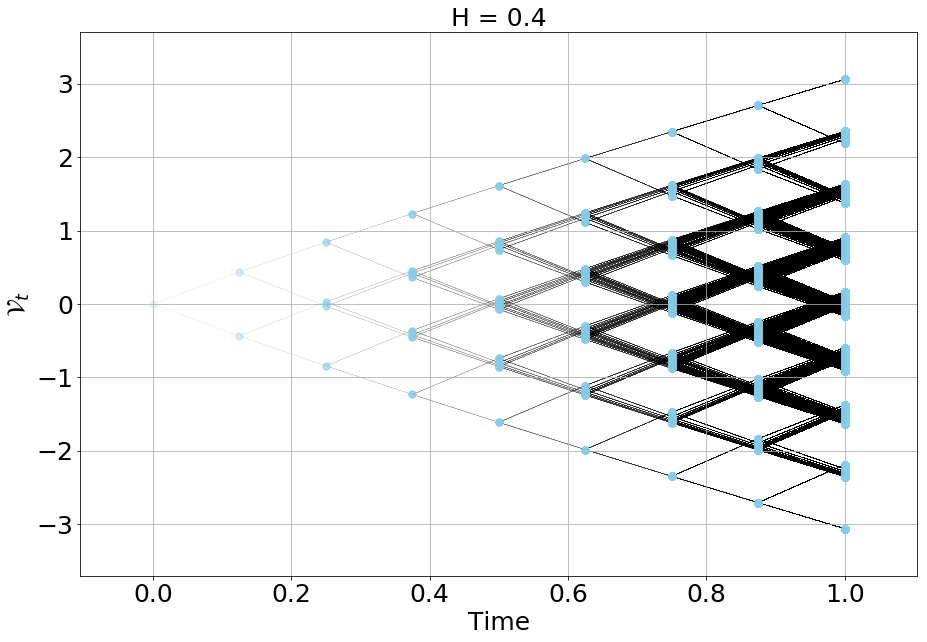
\includegraphics[width=1.0\textwidth]{vol_tree_H04}
    \label{fig:1}
  \end{subfigure}%
  \begin{subfigure}{0.5\textwidth}
    \centering
    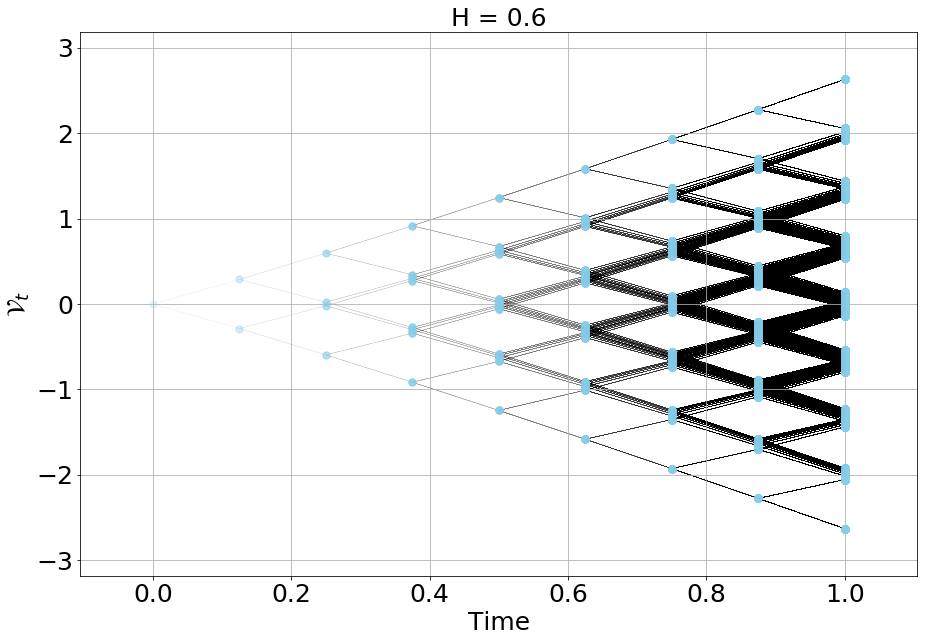
\includegraphics[width=1.0\textwidth]{vol_tree_H06}
    \label{fig:2}
  \end{subfigure}\\
  

  \begin{subfigure}{0.5\textwidth}
    \centering
    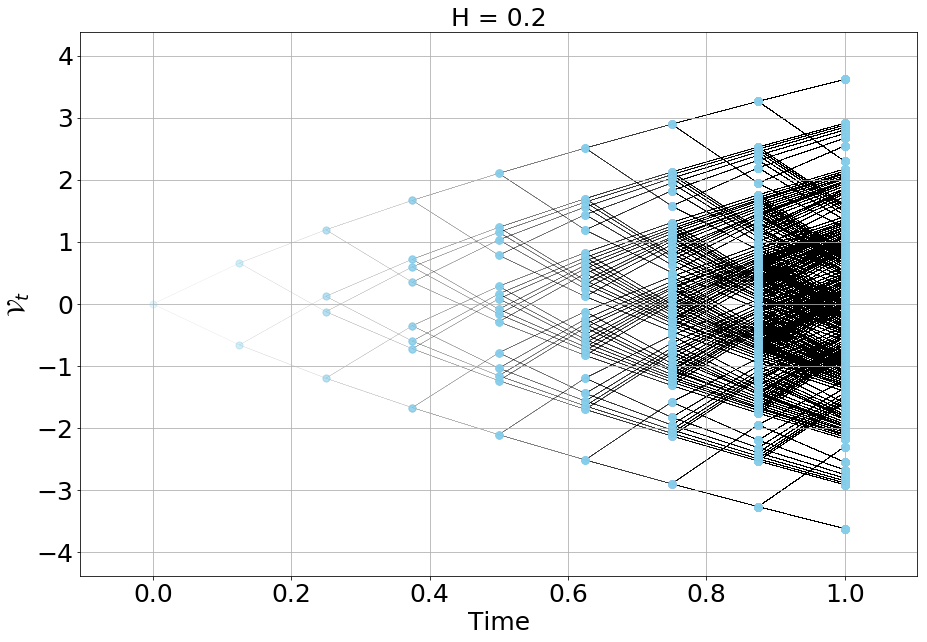
\includegraphics[width=1.0\textwidth]{vol_tree_H02}
    \label{fig:1}
  \end{subfigure}%
  \begin{subfigure}{0.5\textwidth}
    \centering
    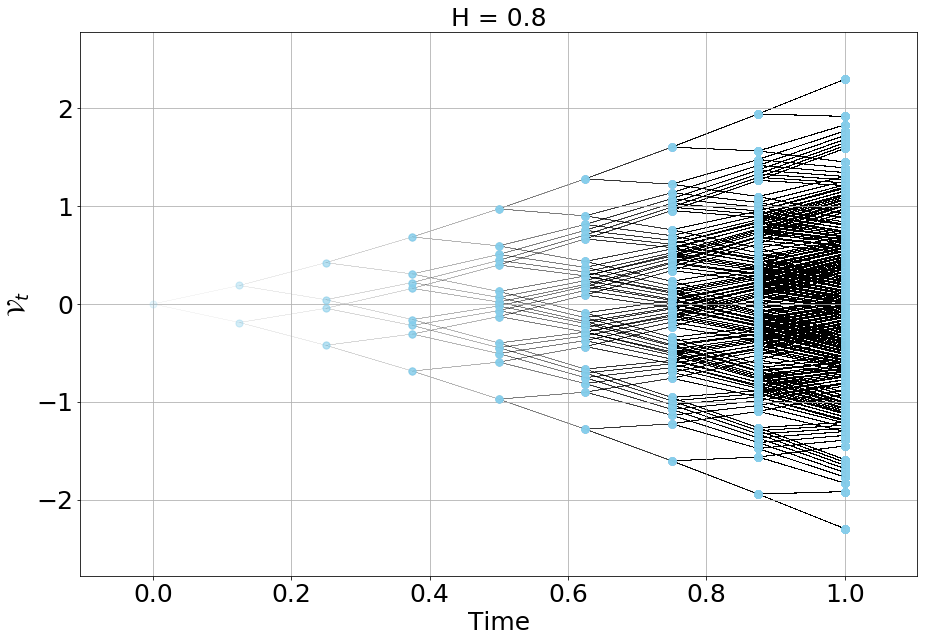
\includegraphics[width=1.0\textwidth]{vol_tree_H08}
    \label{fig:2}
  \end{subfigure}\\
  
  \begin{subfigure}{0.5\textwidth}
    \centering
    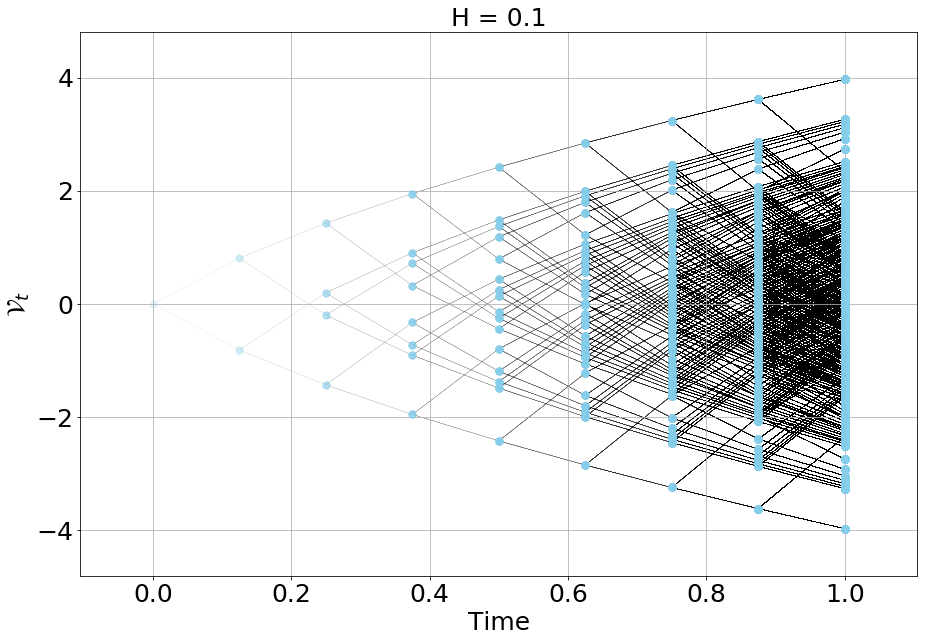
\includegraphics[width=1.0\textwidth]{vol_tree_H01}
    \label{fig:1}
  \end{subfigure}%
  \begin{subfigure}{0.5\textwidth}
    \centering
    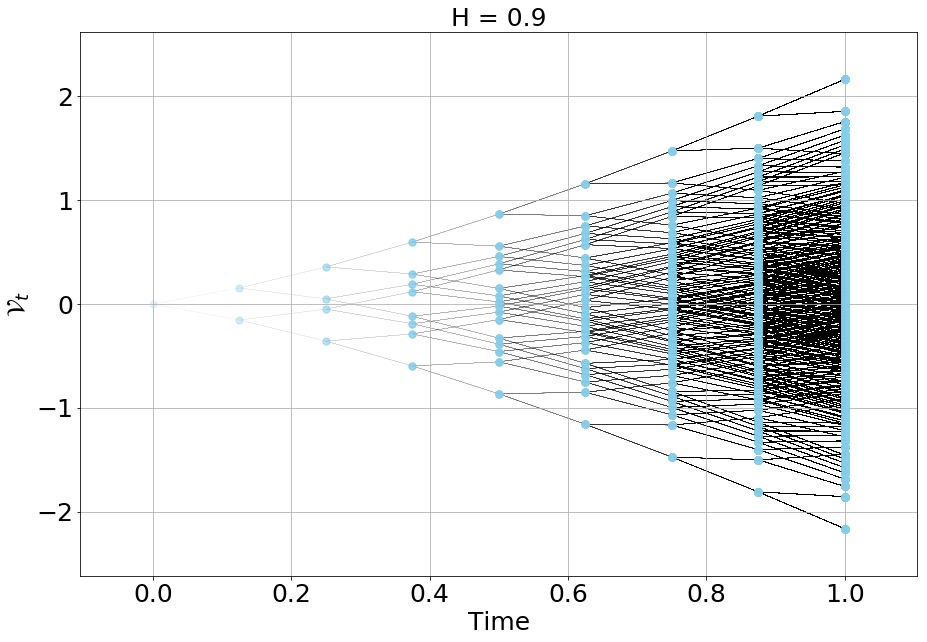
\includegraphics[width=1.0\textwidth]{vol_tree_H09}
    \label{fig:2}
  \end{subfigure}\\
\caption{Logarithmic volatility tree ($T=1, N=8$) with $H<0.5$ on the left and $H>0.5$ on the right. When $H=1/2$, the volatility tree is completely recombining.}
\label{fig:voltree}
\end{center}
\end{figure}

\begin{figure}[htb!]
\begin{center}
  
  \begin{subfigure}{0.5\textwidth}
    \centering
    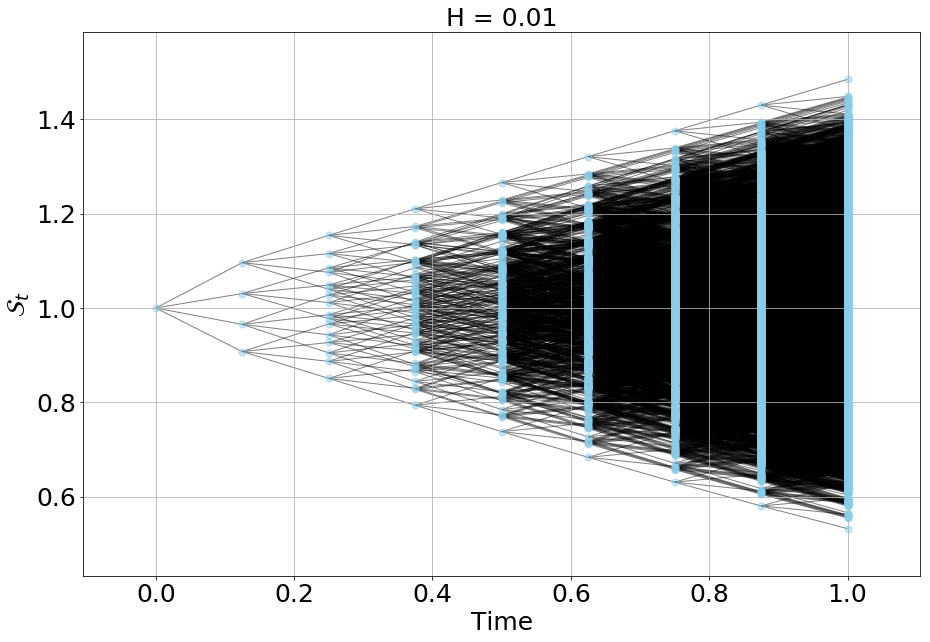
\includegraphics[width=1.0\textwidth]{price_tree_H001}
    \label{fig:1}
  \end{subfigure}%
  \begin{subfigure}{0.5\textwidth}
    \centering
    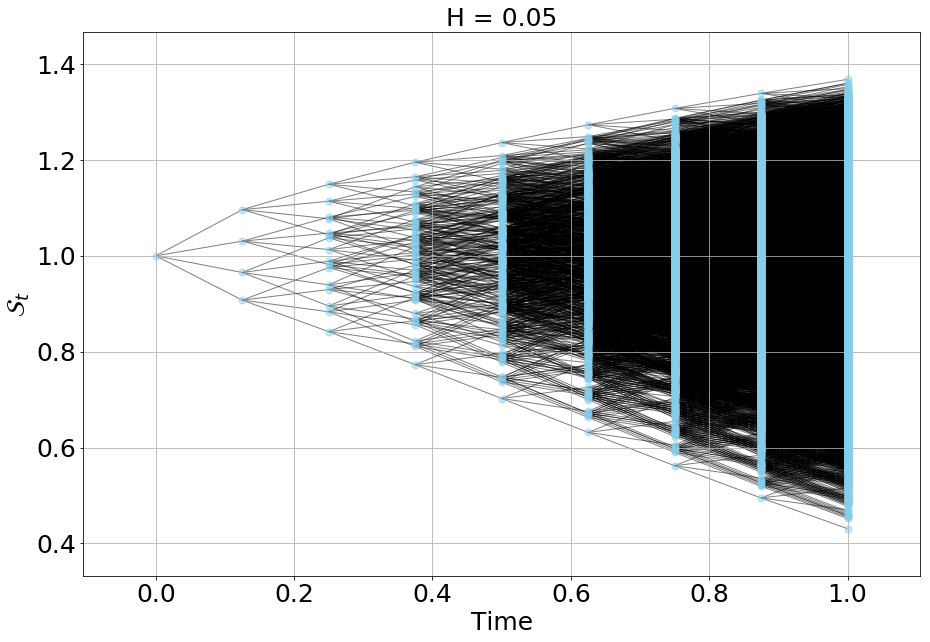
\includegraphics[width=1.0\textwidth]{price_tree_H005}
    \label{fig:2}
  \end{subfigure}\\
  
  \begin{subfigure}{0.5\textwidth}
    \centering
    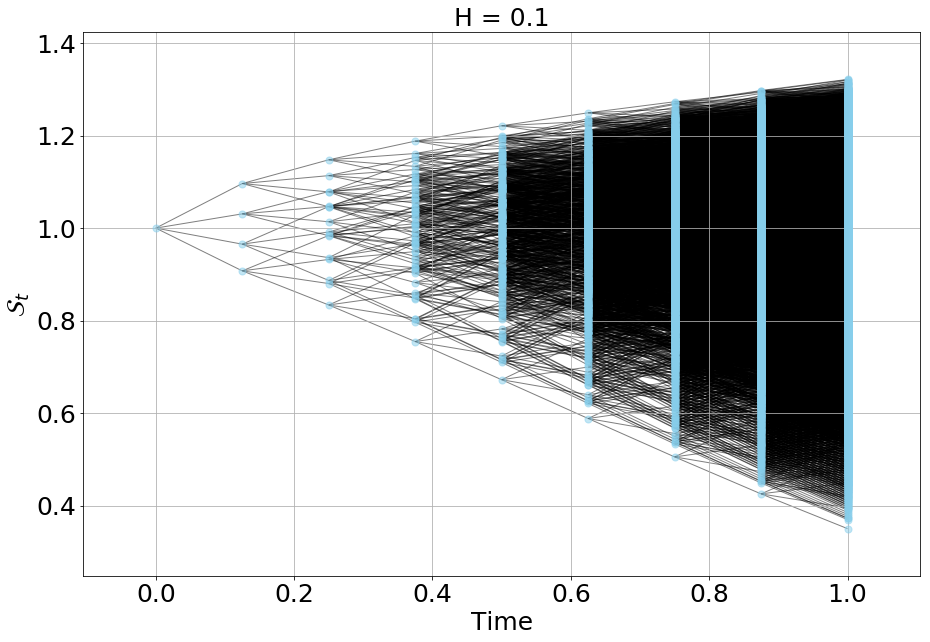
\includegraphics[width=1.0\textwidth]{price_tree_H01}
    \label{fig:1}
  \end{subfigure}%
  \begin{subfigure}{0.5\textwidth}
    \centering
    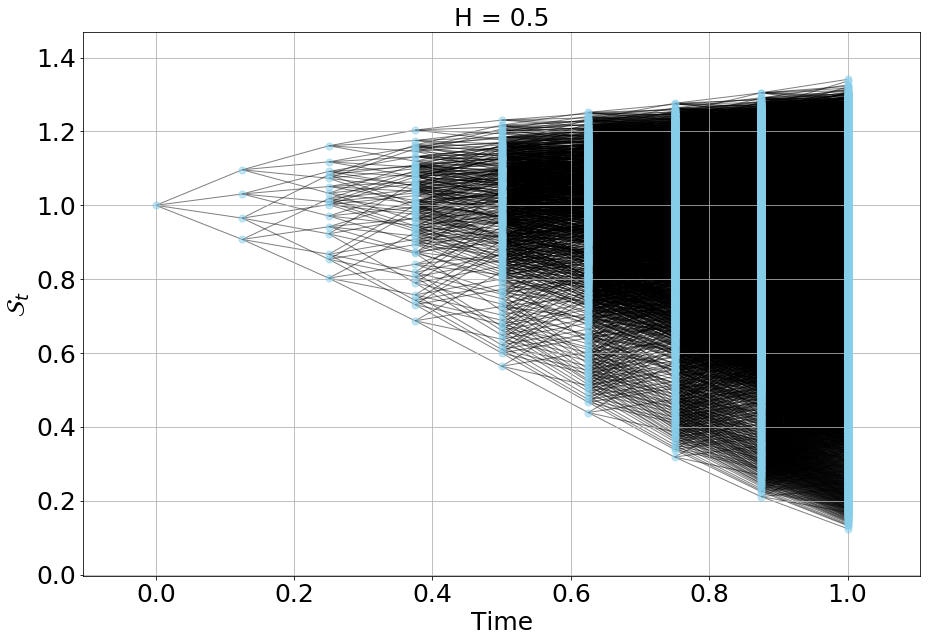
\includegraphics[width=1.0\textwidth]{price_tree_H05}
    \label{fig:2}
  \end{subfigure}\\
  
  \begin{subfigure}{0.5\textwidth}
    \centering
    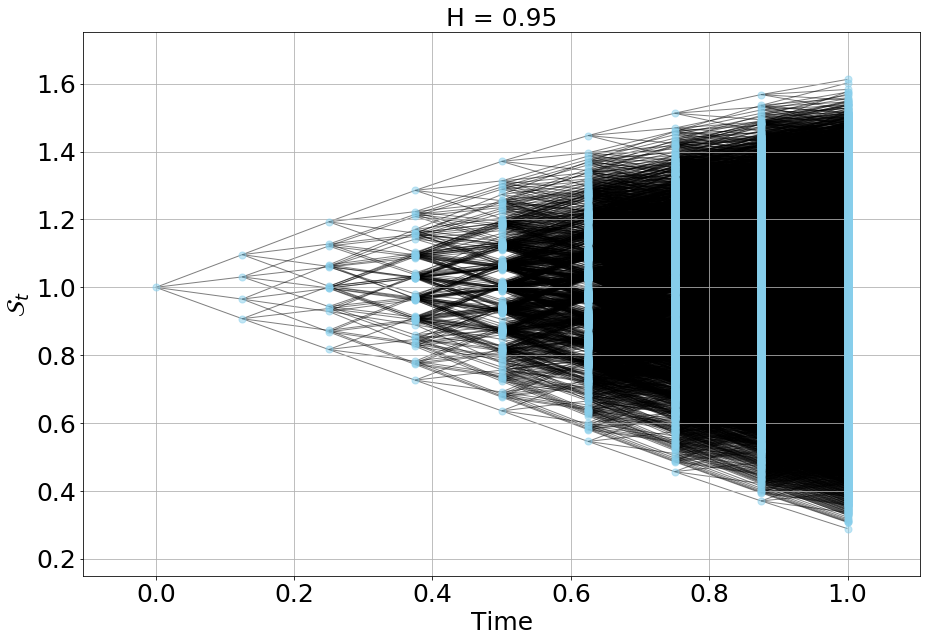
\includegraphics[width=1.0\textwidth]{price_tree_H095}
    \label{fig:1}
  \end{subfigure}%
  \begin{subfigure}{0.5\textwidth}
    \centering
    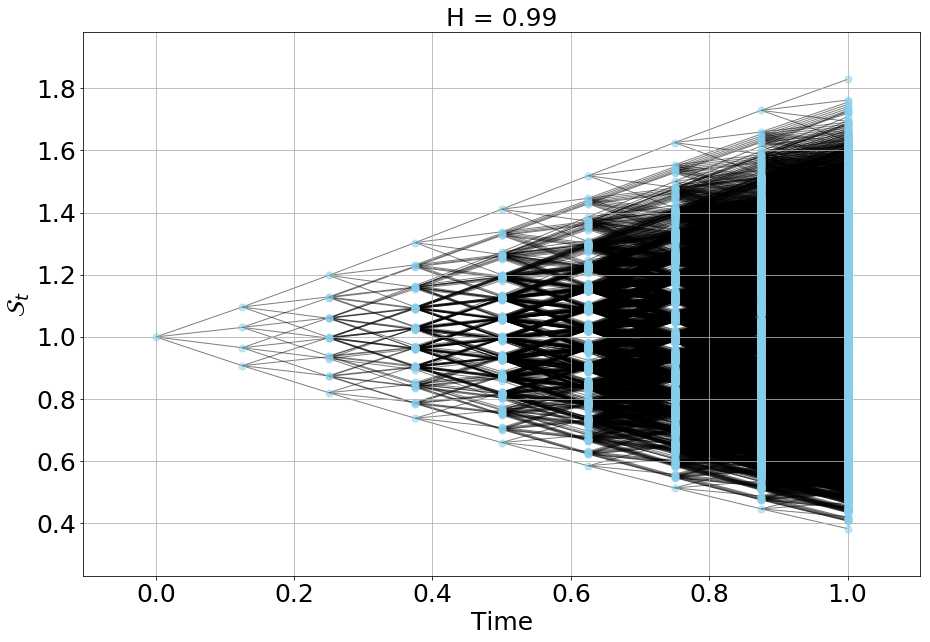
\includegraphics[width=1.0\textwidth]{price_tree_H099}
    \label{fig:2}
  \end{subfigure}\\

\caption{Stock price tree ($T=1, N=8$) with $\nu=1$, $\rho=-0.9$, $\xi_0(t)\equiv 0.04$, $H\in\{0.01, 0.05, 0.1, 0.5, 0.95, 0.99\}$.}
\label{fig:pricetree1}
\end{center}
\end{figure}


\subsection{Example: Analytic Calculation of a Two-Step Tree}
For the purpose of verifying numerical computations in the following section, we perform an analytic calculation in the simple case of a fully (anti)-correlated ($\rho=\pm 1$) two-step tree ($n=2$). Initial condition $X_0=0$. At $1^{\text{st}}$ time step, the volatility is evaluated at $t=0$ using $\mathcal{V}_0 = \xi_0(t=0)\equiv \xi_0$:
\begin{align}
X_1 = \begin{cases}
-\frac{1}{2}\xi_0 \Delta t + \rho \sqrt{\xi_0\Delta t}, \quad \xi_1 = +1,\\
-\frac{1}{2}\xi_0 \Delta t - \rho \sqrt{\xi_0\Delta t}, \quad \xi_1 = -1.
\end{cases}
\end{align}
At $2^{\text{nd}}$ time step, the volatility is evaluated at $t=1$ using $\mathcal{V}_1 =\Delta t^H \xi_1$:
\begin{align}
V_1 = \xi_0 \exp\left( 2\nu C_H \Delta t^H \xi_1 - \frac{\nu^2 C_H^2 \Delta t^{2H}}{H} \right).
\end{align}
Thus,
{
\footnotesize{
\begin{align*}
X_2 = X_1 + \begin{cases}
-\frac{1}{2}\xi_0 \Delta t \cdot e^{+2 \nu C_H \Delta t^H - \frac{\nu^2 C_H^2 \Delta t^{2H}}{H}}
+\rho\sqrt{\xi_0\Delta t} \cdot e^{+\nu C_H \Delta t^H - \frac{\nu^2 C_H^2 \Delta t^{2H}}{2H}}, \quad \xi_1 = +1, \,\xi_2 = +1,\\
-\frac{1}{2}\xi_0 \Delta t \cdot e^{+2 \nu C_H \Delta t^H - \frac{\nu^2 C_H^2 \Delta t^{2H}}{H}}
-\rho\sqrt{\xi_0\Delta t} \cdot e^{+\nu C_H \Delta t^H - \frac{\nu^2 C_H^2 \Delta t^{2H}}{2H}}, \quad \xi_1 = +1, \,\xi_2 = -1,\\
-\frac{1}{2}\xi_0 \Delta t \cdot e^{-2 \nu C_H \Delta t^H - \frac{\nu^2 C_H^2 \Delta t^{2H}}{H}}
+\rho\sqrt{\xi_0\Delta t} \cdot e^{- \nu C_H \Delta t^H - \frac{\nu^2 C_H^2 \Delta t^{2H}}{2H}}, \quad \xi_1 = -1, \,\xi_2 = +1,\\
-\frac{1}{2}\xi_0 \Delta t \cdot e^{-2 \nu C_H \Delta t^H - \frac{\nu^2 C_H^2 \Delta t^{2H}}{H}}
-\rho\sqrt{\xi_0\Delta t} \cdot e^{- \nu C_H \Delta t^H - \frac{\nu^2 C_H^2 \Delta t^{2H}}{2H}}, \quad \xi_1 = -1, \,\xi_2 = -1.
\end{cases}
\end{align*}
}
}\\
The spread between the two nodes at $1^{\text{st}}$ time step is $2\sqrt{\xi_0\Delta t}$ regardless. At $2^{\text{nd}}$ time step, there are four nodes. The spread between the upper two nodes $S_H$ and the spread between the lower two nodes $S_L$ are:
\begin{align}
S_H &= 2\sqrt{\xi_0\Delta t}\cdot e^{-\rho\nu C_H \Delta t^H -\frac{\nu^2 C_H^2 \Delta t^{2h}}{2H}}, \quad S_L &= 2\sqrt{\xi_0\Delta t}\cdot e^{+\rho\nu C_H \Delta t^H -\frac{\nu^2 C_H^2 \Delta t^{2h}}{2H}}
\end{align}
Figure \ref{fig:schematictree} shows a schematic representation of the two-step trees with $\rho=\pm 1$.
\begin{figure}[htb!]
\begin{center}
  \begin{subfigure}{0.5\textwidth}
    \centering
    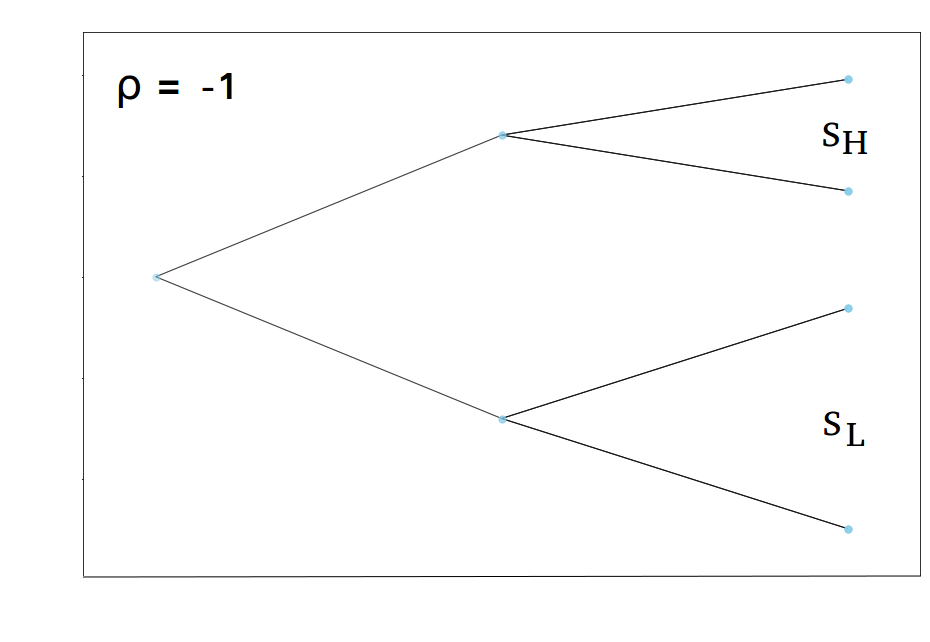
\includegraphics[width=1.0\textwidth, height=5cm]{shsl_1}
    \label{fig:1}
  \end{subfigure}%
  \begin{subfigure}{0.5\textwidth}
    \centering
    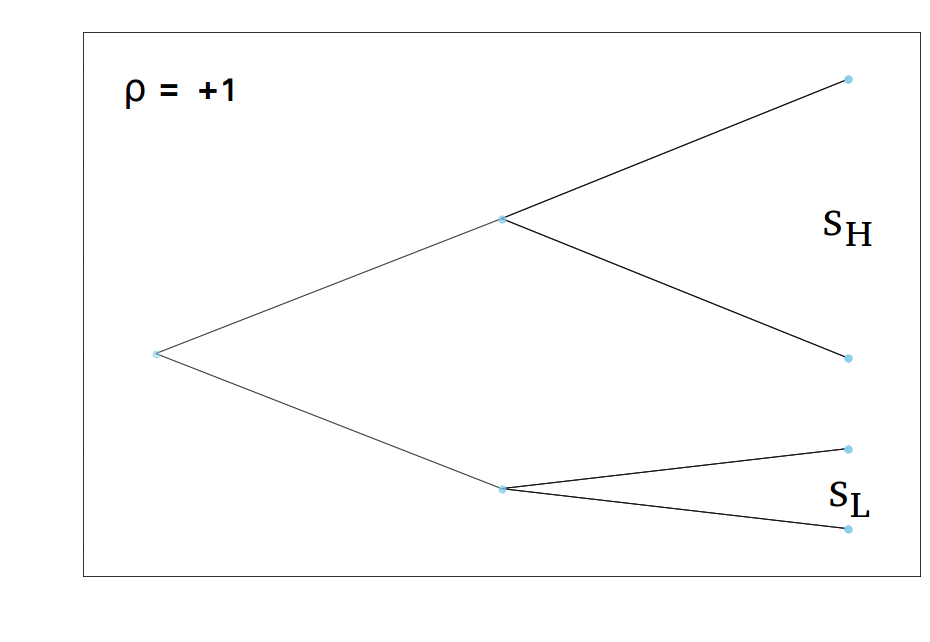
\includegraphics[width=1.0\textwidth, height=5cm]{shsl_2}
    \label{fig:2}
  \end{subfigure}
\caption{Schematic two-step tree: $\rho=-1$ (left) and $\rho=+1$ (right).}
\label{fig:schematictree}
\end{center}
\end{figure}
\newline
The ratio between the upper spread $S_H$ and the lower spread $S_L$ is
\begin{align}
\frac{S_H}{S_L} = e^{2\rho\nu C_H \Delta t^H}.
\end{align}
The two-step model captures the important feature that the tree is tilted downward when $\rho=-1$ and tilted upward when $\rho=+1$. When the price and vol is anti-correlated, the subtree span is inversely related to the subtree level; when the price and vol is positively correlated, the subtree span is positively related to the subtree level.


\section{Results I: European Put Options}
\label{euputoptions}
In this section, for a range of moneyness and a fixed time to expiration, we evaluate the European put options in two models:
\begin{itemize}[noitemsep]
\item rBergomi model, using the quadrinomial tree implementation in Section \ref{rbergomitree};
\item local volatility model, using the binomial implied tree introduced in \cite{derman}.
\end{itemize}
We calibrate the local volatility model to the same smile generated by rBergomi model --- for the purpose of further comparing the American put options and the associated early exercise premium calculated in the two models within a common framework. We delibrately choose the implied tree of Derman and Kani \cite{derman} to implement the local volatility model to be consistent in style. The following parameters are used in calculation:
\begin{itemize}[noitemsep]
\item Intereste rate: $r=0$;
\item Vol of vol: $\nu = 1.0$;
\item Spot-vol correlation: $\rho = -0.9$;
\item Roughness: $H = 0.05$;
\item Flat forward variance curve: $\xi_0(t)\equiv 0.04$, $\forall t>0$.
\item Time to expiration: $T=1$;
\item Moneyness: $\log\frac{K}{S} \in (-0.3, + 0.3)$;
\item Number of time steps (rBergomi tree and implied volatility tree): $N=10$.
\end{itemize}
The result is shown in Figure \ref{fig:euput}. The upper panel shows the rBergomi tree (a quadrinomial tree) and the calibrated implied volatility tree (a distorted binomial tree). The lower panel shows the European put option prices as a function of logarithmic moneyness. As expected, the local volatility model generated by Derman and Kani \cite{derman} is calibrated to the same smile generated by the rBergomi model. This ensures that the local volatility model is consistent with the rBergomi model it calibrates to and further calculations for American options are comparable. For a market where the vanilla options are traded, it is important to impose the constraint of fixing European option prices by those given by the market while one examines the dependence of non-vanilla options on the model parameters. 

\begin{figure}
\begin{center}
  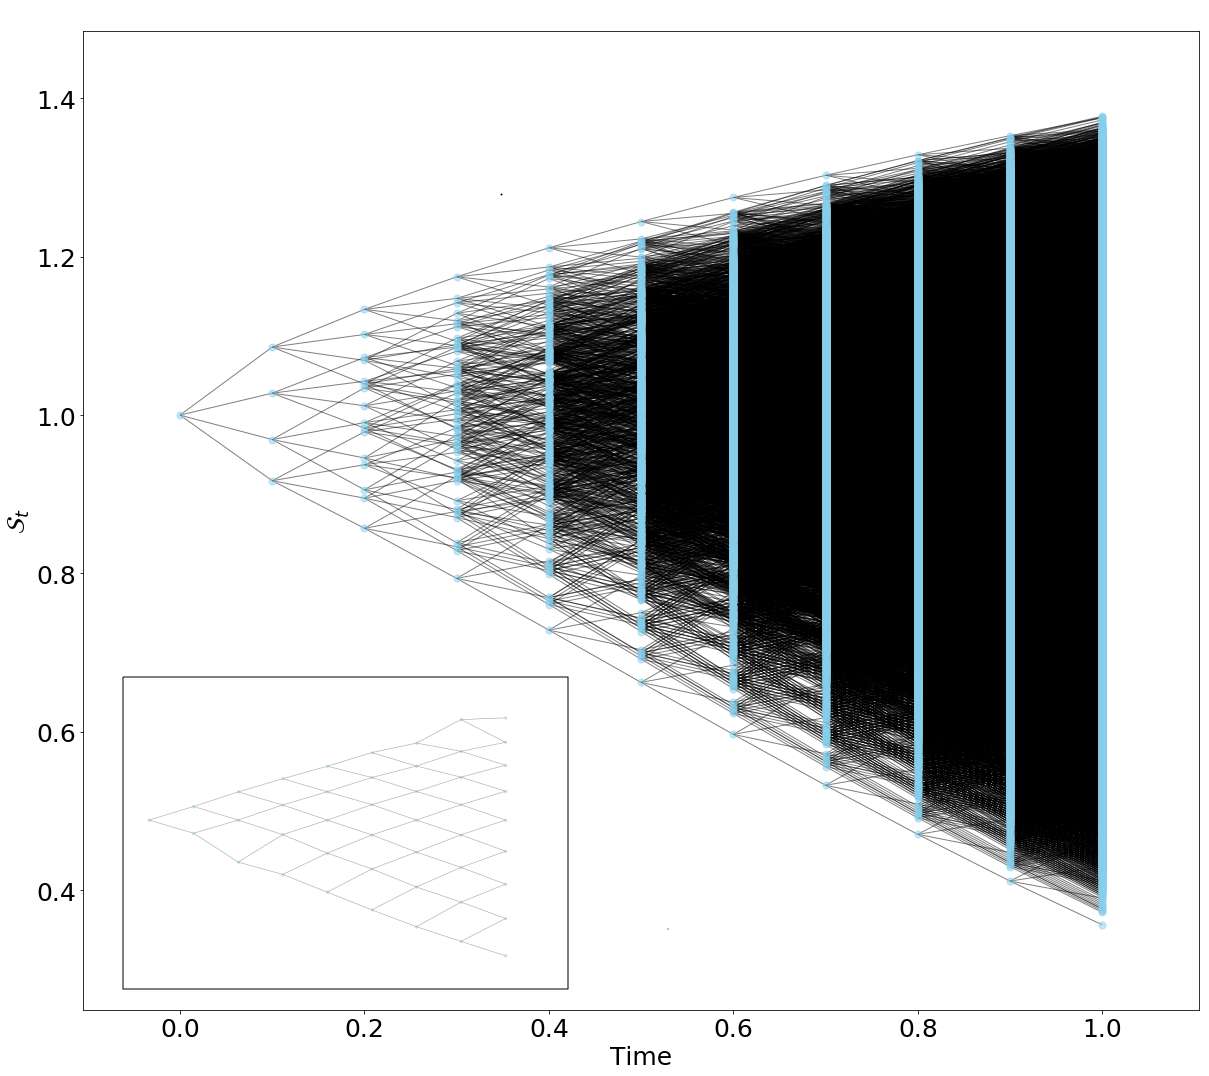
\includegraphics[width=0.8\textwidth, height=9cm]{big_price_tree}
  \vadjust{\vskip 10mm \vskip 0pt}
  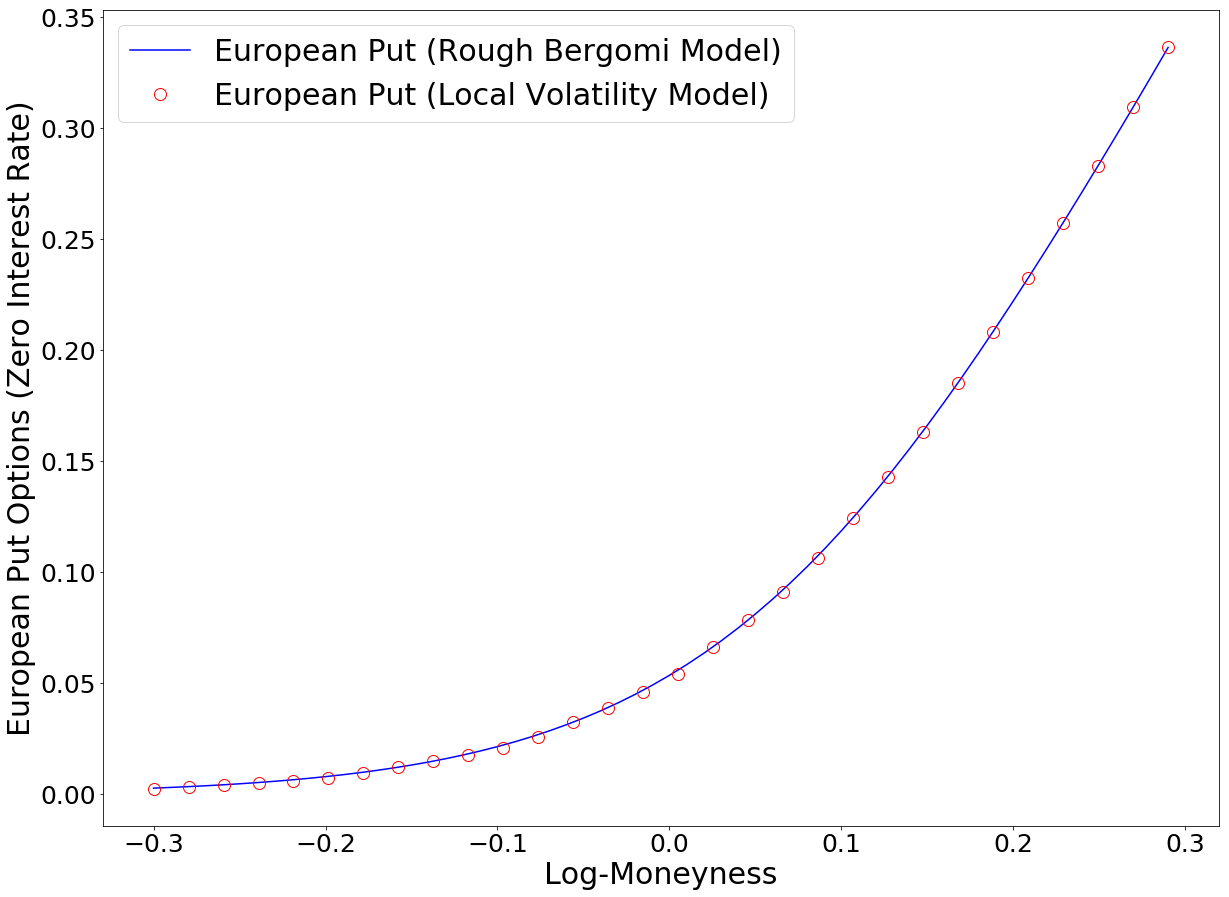
\includegraphics[width=0.8\textwidth, height=9cm]{euput}
\caption{Upper panel: rBergomi tree with $N=10$ time steps; inset: implied local volatility tree. Lower panel: European put option prices as a function of logarithmic moneyness, in rBergomi tree model (blue line) and local volatility model (red circle) calibrated to the same smile using Derman and Kani \cite{derman}. Good agreement is observed.}
\label{fig:euput}
\end{center}
\end{figure}

\newpage

\section{Results II: Early Exercise Premium (EEP)}
In this section, for a range of moneyness and a fixed time to expiration, we evaluate the early exercise premium $\text{EEP}(K,T) \triangleq \text{American Put}(K,T) - \text{European Put}(K,T)$ in two models constructed in Section \ref{euputoptions}, where the local volatility model is calibrated to the same smile generated by rBergomi model. The following parameters are used:
\begin{itemize}[noitemsep]
\item Intereste rate: $r=5\%$;
\item Vol of vol: $\nu = 1.0$;
\item Spot-vol correlation: $\rho = -0.9$;
\item Roughness: $H = 0.05$;
\item Flat forward variance curve: $\xi_0(t)\equiv 0.04$, $\forall t>0$.
\item Time to expiration: $T=1$;
\item Moneyness: $\log\frac{K}{S} \in (-0.3, + 0.3)$;
\item Number of time steps (rBergomi tree and implied volatility tree): $N=10$.
\end{itemize}
The result is shown in Figure \ref{fig:eep}. We observe that, in the early exercise premium, the largest discrepancy between the rBergomi model and the calibrated local volatility model occurs for intermediate strike values $\log\frac{K}{S}\approx 10\%$. In the limiting case where the put option is deeply in-the-money, the early exercise premium increases in magnitude in both models but the discrepancy diminishes.

\begin{figure}[!htb]
\begin{center}
  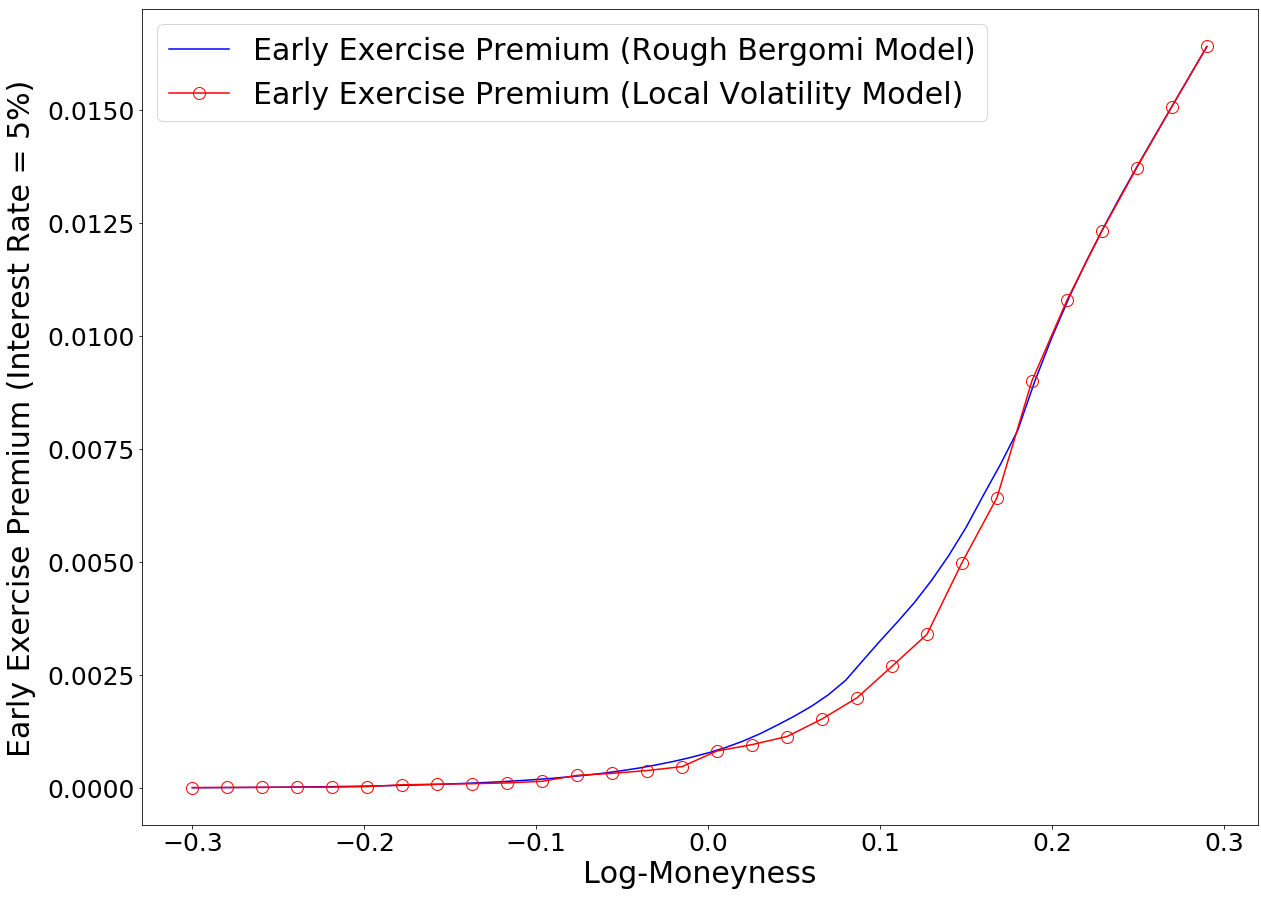
\includegraphics[width=0.75\textwidth, height=8.5cm]{eep}
\caption{Early exercise premium of American put options as a function of logarithmic moneyness, in rBergomi model (blue line) and local volatility model (red circle) calibrated to the same European smile generated by rBergomi model.}
\label{fig:eep}
\end{center}
\end{figure}


\section{Results III: EEP and Model Parameters}
In this section, we examine the dependence of early exercise premium on the rBergomi model parameters. In particular, (1) vol of vol: $\nu>0$; (2) spot-vol correlation: $\rho \in [-1,1]$; (3) roughness: $H \in [0,1/2]$. We leave the dependence on forward variance curve, assumed to be flat in this report, for future research. We assess the effects on early exercise premium relative to a local volatility model, calibrated to the same European volatility smile generated by rBergomi model. To fix notations, denote the early exercise premium of an American option struck at $K$ and maturing at $T$, relative to a local volatility model, by
\begin{align}
\mathbb{EEP}(K,T) \triangleq \text{EEP}^{\text{rBergomi}}(K,T) - \text{EEP}^{\text{Local Vol}}(K,T).
\end{align}
We measure the relative early exercise premium aggregated across the volatility smile for a fixed maturity $T$ by
\begin{align*}
\mathbb{EEP}(T) \triangleq \int_0^\infty \mathbb{EEP}(K,T) \frac{dK}{K} \approx \sum_{i} \mathbb{EEP}(K_i,T)\Delta \log K_i = \Delta \sum_{i} \mathbb{EEP}(K_i,T),
\end{align*}
where we sampled the strikes in equal-spacing logarithmic moneyness $\Delta \log K_i \equiv \Delta$.

\subsection{$\mathbb{EEP}$ and Vol of Vol: $\nu$ ($\rho$ and $H$ fixed)}
\begin{figure}[!htb]
\begin{center}
  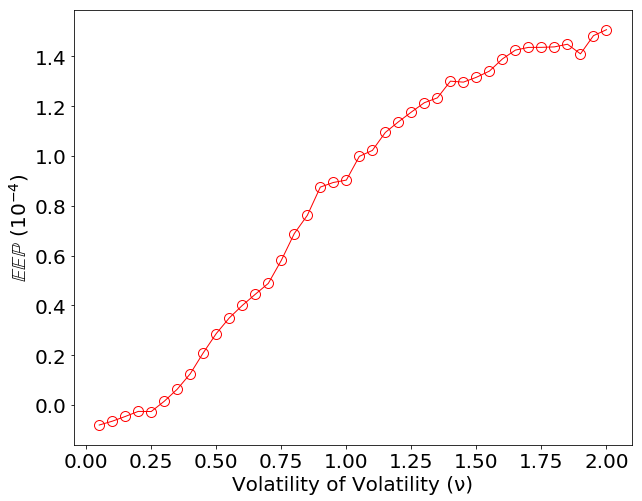
\includegraphics[width=0.75\textwidth, height=8.5cm]{eep_vv}
\caption{$\mathbb{EEP}$ in terms of vol of vol $\nu$ ($T=1$, $H=0.05$, $\rho=-0.9$, $N=10$).}
\label{fig:eep_vv}
\end{center}
\end{figure}
We show in Figure \ref{fig:eep_vv} that the early exercise premium relative to local volatility model, aggregated over logarithmic moneyness $-0.2\le\log \frac{K}{S_0}\le +0.2$, increases with the parameter of volatility of volatility $\nu$, with the other two rBergomi parameters ($H$, $\rho$) fixed. In this limiting case $\nu = 0$, the stochastic volatility model (rBergomi in this work) reduces to local volatility model and the early exercise premium relative to local volatility goes to zero. Intuitively, when the stock price and volatility is assumed to be anti-correlated, a put option currently in-the-money (low stock price) is more likely to get out-of-the-money if the volatility of volatility is high. As a consequence, exercising early is preferable for the holder of an American put option, causing the early exercise premium to increase.

%\subsection{$\mathbb{EEP}$ and Effective Vol of Vol: $\tilde{\eta}\triangleq 2\nu C_H$ ($\rho$ and $H$ fixed)}

\subsection{$\mathbb{EEP}$ and Spot-Vol Correlation: $\rho$ ($\nu$ and $H$ fixed)}
\begin{figure}[!htb]
\begin{center}
  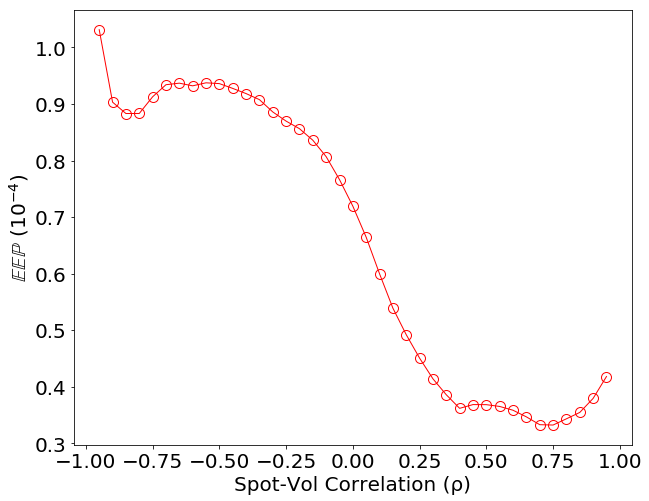
\includegraphics[width=0.75\textwidth, height=8.5cm]{eep_rho}
\caption{$\mathbb{EEP}$ in terms of spot-vol correlation $\rho$ ($T=1$, $H=0.05$, $\nu=1$, $N=10$).}
\label{fig:eep_rho}
\end{center}
\end{figure}
We show in Figure \ref{fig:eep_rho} the early exercise premium relative to local volatility model, aggregated over logarithmic moneyness $-0.2\le\log \frac{K}{S_0}\le +0.2$ in terms of the parameter of spot-vol correlation $\rho$, with the other two rBergomi parameters ($H$, $\nu$) fixed. Generally speaking, the aggregated early exercise premium is observed to decrease as the spot-vol correlation increases. This phenomena can be intuitively understood in terms of the rBergomi tree structure. As the spot price and volatility gets increasingly anti-correlated ($0>\rho\rightarrow -1$), a put option currently in-the-money (low stock price) is more likely to get out-of-the-money because of the associated high volatility. As a consequence, exercising early is preferable for the holder of an American put option, causing the early exercise premium to increase. On the other hand, as the price and volatility gets increasingly correlated ($0<\rho\rightarrow +1$), a put option currently in-the-money (low stock price) at the same time experiences low volatility. As a consequence, the holder of an American put option is less motivated to exercise early, causing the early exercise premium to decrease.

\subsection{$\mathbb{EEP}$ and Roughness: $H$ ($\nu$ and $\rho$ fixed)}
\begin{figure}[!htb]
\begin{center}
  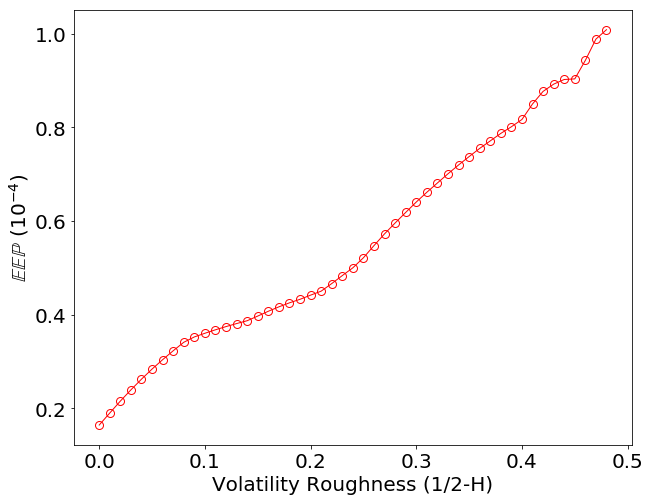
\includegraphics[width=0.75\textwidth, height=8.5cm]{eep_H}
\caption{$\mathbb{EEP}$ in terms of vol roughness $\frac{1}{2}-H$ ($T=1$, $\rho=-0.9$, $\nu=1$, $N=10$).}
\label{fig:eep_H}
\end{center}
\end{figure}
We show in Figure \ref{fig:eep_H} the early exercise premium relative to local volatility model, aggregated over logarithmic moneyness $-0.2\le\log \frac{K}{S_0}\le +0.2$ in terms of the volatility roughness parameter $\gamma\triangleq \frac{1}{2}-H$, with the other two rBergomi parameters ($\rho$, $\nu$) fixed. As expected, the aggregated early exercise premium is observed to increase as the volatility roughness increases. Intuitively spreaking, the rougher the volatility process, the more anti-correlated it is with the stock price process. Thus, a put option currently in-the-money (low stock price resulting from negative price returns) is more likely to get out-of-the-money because of the anti-correlation. As a consequence, exercising early is preferable for the holder of an American put option, causing the early exercise premium to increase.

\subsection{$\mathbb{EEP}$ and Roughness: $H$ ($\tilde{\eta}\triangleq 2\nu C_H$ and $\rho$ fixed)}

Because the combination $2\nu C_H$ (denoted by $\eta\sqrt{2H}$ in Bayer \textit{et. al.}\cite{bayer}) appears naturally in the specification of rBergomi model Eq.(\ref{spec22}), we show in Figure \ref{fig:eep_H_fixed_eta} the early exercise premium relative to local volatility model, aggregated over logarithmic moneyness $-0.2\le\log \frac{K}{S_0}\le +0.2$ in terms of the volatility roughness parameter $\gamma\triangleq \frac{1}{2}-H$, but with $\tilde{\eta} \triangleq 2\nu C_H = \eta\sqrt{2H}$ (as well as the correlation parameter $\rho$) fixed.

\begin{figure}[!htb]
\begin{center}
  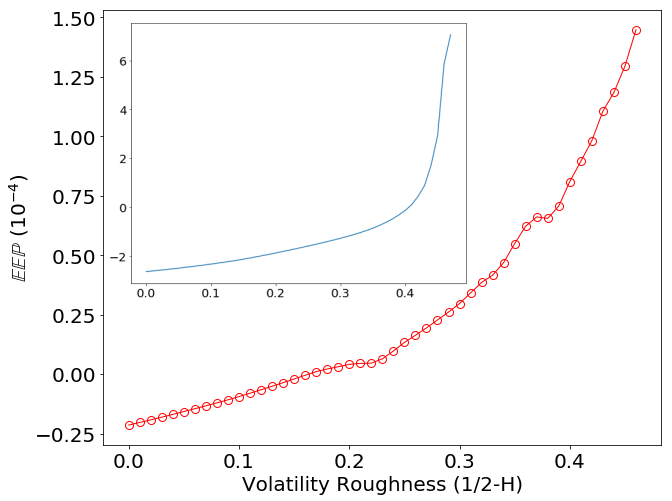
\includegraphics[width=0.75\textwidth, height=8.5cm]{eep_H_fixed_eta}
\caption{$\mathbb{EEP}$ in terms of vol roughness $\frac{1}{2}-H$ ($T=1$, $\rho=-0.9$, $\tilde{\eta} = 0.7$, $N=10$). Inset: At-the-money $\mathbb{EEP}(K/S=1,T)$.}
\label{fig:eep_H_fixed_eta}
\end{center}
\end{figure}

We notice that, in this case, when the roughness gets close to zero $1/2-H \lessapprox 0.15$ and the vol of vol is correspondingly reduced (because $\tilde{\eta}$ fixed), a negative early exercise premium relative to the associated local volatility model is observed.

\section{Summary and Conclusions}
In this report, we calculated the early exercise premium of American put options in rBergomi model and systematically examined its dependence on model parameters. The results are compared to local volatility model calibrated to the same European vanilla smile generated by rBergomi model. The calculations are performed within the tree framework: (1) a quadrinomial tree implementation of rBergomi model \cite{horvath}; (2) the binomial implied volatility tree implementation of Derman and Kani \cite{derman}. We observe that, for $\nu=1.0$, $\rho=\-0.9$, $H=0.05$, $T=1$:
\begin{itemize}[noitemsep]
\item Early exercise premium in rBergomi model is consistently higher than in local volatility model, indicating that rough volatility carries more risk premium;
\item In the limiting cases of deeply in-the-money and deeply out-of-the-money, rBergomi model and the associated local volatility model give the same early exercise premium for American put options;
\item The largest discrepancy in early exercise premium between rBergomi model and local volatility model occurs when the logarithmic moneyness $\log\frac{K}{S}\approx 10\%$.
\end{itemize}
In prior literature, the model parameters are tuned to assess the effects on the early exercise premium, ignoring that this also changes the prices of European options. In this work, instead, we systematically examine the early exercise premium relative to a local volatility model, calibrated to the same European volatility smile generated by rBergomi model: $\mathbb{EEP} \triangleq \text{EEP}^{\text{rBergomi}} - \text{EEP}^{\text{Local Vol}}$. By constraining to the same European volatility smile, we remove the part of changes in early exercise premium that are associated with changes in European option prices. We observe that, the early exercise premium relative to local volatility model, aggregated over logarithmic moneyness $-0.2\le\log \frac{K}{S_0}\le +0.2$, 
\begin{itemize}[noitemsep]
\item increases with the parameter of volatility of volatility $\nu$, with the other two rBergomi parameters ($H$, $\rho$) fixed;
\item decreases as the spot-vol correlation increases (mostly, $-3/4\le \rho \le +3/4$), with the other two rBergomi parameters ($H$, $\nu$) fixed;
\item increase as the volatility roughness increases, with the other two rBergomi parameters ($\rho$, $\nu$) fixed.
\end{itemize}

%%%%%%%%%%%%%%%%%%%%%%%%%%%%%%%%%%%%%%%%%%%%%%%%%%%%%%%%%%%%%%%%%%%%%%%%%%%%%%%%%%%%%%%%
%
%
%  Bibliography
%
%
%%%%%%%%%%%%%%%%%%%%%%%%%%%%%%%%%%%%%%%%%%%%%%%%%%%%%%%%%%%%%%%%%%%%%%%%%%%%%%%%%%%%%%%%

\begin{thebibliography}{}

\bibitem{gatheral1} {J. Gatheral, T. Jaisson, and M. Rosenbaum},
{Volatility is Rough},
{\textit{Quantitative Finance}} (2018).

\bibitem{bayer} { C. Bayer, P. Friz, and J. Gatheral},
{Pricing under Rough Volatility},
{\textit{Quantitative Finance}} (2016).

\bibitem{jacquier1} { A. Jacquier, C. Martini, and A. Muguruza},
{On VIX Futures in the Rough Bergomi Model},
{\textit{arXiv:1701.04260}} (2017).

\bibitem{horvath} { B. Horvath, A. Jacquier, and A. Muguruza},
{Functional Central Limit Theorems for Rough Volatility},
{\textit{arXiv:1711.03078}} (2017).

\bibitem{derman} { E. Derman and I. Kani},
{The Volatility Smile and Its Implied Tree},
{\textit{Goldman Sachs Quantitative Strategies Research Notes}} (1994).


\end{thebibliography}

\newpage

%\appendix

%\section{\large{Characteristic Correlator of Fractional Brownian Motion}}
%\label{integralrepresentations}

%The characteristic correlator of fractional Brownian motion ($0<H<1$) is
%\begin{align*}
%\mathbb{E}[W^H_s W^H_t] &= \frac{1}{2}\mathbb{E}\left[ (W^H_s)^2 + (W^H_t)^2 - (W^H_s - W^H_t)^2 \right]\\
%&= \frac{1}{2}\mathbb{E}\left[ (W^H_s)^2 + (W^H_t)^2 - (W^H_{s-t})^2\right]\\
%&= \frac{\rho(H)}{2}\left( s^{2H} + t^{2H} - |s-t|^{2H} \right),
%\end{align*}
%where $\rho(H)\triangleq \mathbb{E}[(W_1^H)^2]$. An integral representation of fractional Brownian motion is written as
%$$
%W^H_t = \int_{\mathbb{R}} K(t,s)dW_s,
%$$
%where $W_s = W^{1/2}_s$ denotes standard Brownian motion and $K(t,s)$ is the kernel. Mandelbrot-van Ness representation chooses
%$$
%K(t,s) \triangleq \kappa(H)\left[ (t-s)_+^{H-1/2} - (-s)_+^{H-1/2} \right].
%$$
%Then the normalization constants $\rho(H)$ of the correlator and $\kappa(H)$ of the kernel are related by
%$$
%\rho(H) = \kappa^2(H) \frac{3/2-H}{2H}B(2-2H, H+1/2),
%$$
%where the beta function $B(\alpha,\beta) = \int_0^1 t^{\alpha-1}(1-t)^{\beta-1}dt = \frac{\Gamma(\alpha)\Gamma(\beta)}{\Gamma(\alpha+\beta)}$, $\alpha>0, \beta>0$.\\
%\newline
%\textit{Proof}: Compute the variance of fractional Brownian motion
%\allowdisplaybreaks
%\begin{align*}
%&\quad \mathbb{E}\left[ \left( \int_{-\infty}^t (t-s)^{H-1/2}dW_s - \int_{-\infty}^0 (-s)^{H-1/2}dW_s \right)^2 \right]\\
%&= \int_{-\infty}^t\int_{-\infty}^t  (t-s)^{H-1/2}(t-u)^{H-1/2} \mathbb{E}[dW_s dW_u]\\
%&\quad -2\int_{-\infty}^t\int_{-\infty}^0 (t-s)^{H-1/2}(-u)^{H-1/2}\mathbb{E}[dW_s dW_u]\\
%&\quad + \int_{-\infty}^0\int_{-\infty}^0 (-s)^{H-1/2}(-u)^{H-1/2} \mathbb{E}[dW_s dW_u]\\
%&= \int_{-\infty}^t (t-s)^{2H-1} ds - 2\int_{-\infty}^0 (t-s)^{H-1/2}(-s)^{H-1/2}ds + \int^{0}_{-\infty} s^{2H-1}ds\\
%&= \int^{\infty}_0 (t+s)^{2H-1} ds + \int_{0}^t (t-s)^{2H-1}ds - 2\int^{\infty}_0 (t+s)^{H-1/2}s^{H-1/2}ds + \int_{0}^{\infty} s^{2H-1}ds\\
%&= \int_0^\infty \left[ (t+s)^{H-1/2} - s^{H-1/2} \right]^2 ds  + \int_{0}^t (t-s)^{2H-1}ds\\
%&= \underbrace{\int_0^\infty \left[ (t+s)^{H-1/2} - s^{H-1/2} \right]^2 ds}_{\triangleq \phi(t)}  + t^{2H }\int_{0}^1 (1-x)^{2H-1}dx\\
%&= \phi(t)  + \frac{t^{2H }}{2H}.
%\end{align*}
%Next, evaluate $\phi(t)$. Note that $\phi(0)=0$. Keep differentiating (twice), remember $H-1<0$:
%\allowdisplaybreaks
%\begin{align*}
%\phi'(t) &= (2H-1)\int_0^\infty \left[ (t+s)^{2H-2}- (t+s)^{H-3/2}s^{H-1/2} \right]ds, \quad \text{Note: } \phi'(0)=0,\\
%\phi''(t) &= (2H-1)\int_0^\infty \left[ (2H-2)(t+s)^{2H-3} - (H-3/2)s^{H-1/2}(t+s)^{H-5/2} \right]ds\\
%&= (2H-1)(2H-2)\int_0^\infty (t+s)^{2H-3}ds - (2H-1)(H-3/2)\int_0^\infty s^{H-1/2}(t+s)^{H-5/2}ds\\
%&= -(2H-1)t^{2H-2} - (2H-1)(H-3/2)t^{2H-2}\int_0^\infty x^{H-1/2}(1+x)^{H-5/2}dx\\
%&= -(2H-1)t^{2H-2} - (2H-1)(H-3/2)t^{2H-2}\int_1^\infty (y-1)^{H-1/2}y^{H-5/2}dy\\
%&= -(2H-1)t^{2H-2} - (2H-1)(H-3/2)t^{2H-2}\int_1^0 \left(\frac{1}{z}-1\right)^{H-1/2}z^{5/2-H}\left(-\frac{dz}{z^2}\right)\\
%&= -(2H-1)t^{2H-2} - (2H-1)(H-3/2)t^{2H-2}\int_0^1 z^{(2-2H)-1}(1-z)^{(H+1/2)-1}dz\\
%&= -(2H-1)t^{2H-2} - (2H-1)(H-3/2)t^{2H-2}B(2-2H, H+1/2).
%\end{align*}
%Next integrate twice, and use $\phi(0)=0, \phi'(0)=0$:
%\begin{align*}
%\phi(t) = -\frac{t^{2H}}{2H} &+ \frac{t^{2H}}{2H}(3/2-H)B(2-2H, H+1/2)\\
%\Rightarrow \phi(t) + \frac{t^{2H}}{2H} &= t^{2H} \frac{(3/2-H)\Gamma(2-2H)\Gamma(H+1/2)}{2H\times\Gamma(5/2-H)} = t^{2H} \frac{\Gamma(2-2H)\Gamma(H+1/2)}{2H\times%\Gamma(3/2-H)}.
%\end{align*}
%Thus,
%\begin{align*}
%&\quad \mathbb{E}\left[ (W^H_t)^2 \right] = \kappa^2(H)t^{2H}  \frac{\Gamma(2-2H)\Gamma(H+1/2)}{2H\times\Gamma(3/2-H)} \Rightarrow \rho(H) = \kappa^2(H) \frac{\Gamma(2-2H)\Gamma(H+1/2)}{2H\times\Gamma(3/2-H)}.
%\end{align*}
%Two common choices are:\\
%\newline
%(1) $\rho(H)\equiv 1$ (Jost 2008), then
%$$
%\kappa(H) = \sqrt{\frac{2H\times\Gamma(3/2-H)}{\Gamma(2-2H)\Gamma(H+1/2)}};
%$$
%(2) $\kappa(H) \triangleq \frac{1}{\Gamma(H+1/2)}$ (Mandelbrot-van Ness 1968), then
%$$
%\rho(H) = -2\frac{\cos(\pi H)}{\pi}\Gamma(-2H),
%$$
%where some properties of $\Gamma$ function are used to derive the above expression; also, $\rho(H=1/2)=1$, consistent with standard Brownian motion.

%\section{\large{Numerical Data Structure of Non-Recombining Tree}}
%\label{treedatastructure}
%A quadrinomial tree with $N$ time steps has
%$$
%\text{Total number of nodes } = \frac{4^{N+1}-1}{3}.
%$$ 
%At the $N^{\text{th}}$ time step, it has
%$$
%\text{Number of nodes at } N^{\text{th}} \text{ time step } = 4^N.
%$$
%Each node in tree at the $n^{\text{th}}$ time step, where $0\le n\le N$ is encoded by a sequence
%$$
%(i_1, i_2, \cdots, i_n),
%$$
%where each $i\in\{0,1,2,3\}$. This sequence is naturally mapped to an integer
%$$
%(i_1, i_2, \cdots, i_n) \Longleftrightarrow I_n = i_1\times 4^{n-1} + i_2\times 4^{n-2} + \cdots + i_{n-1}\times 4 + i_n.
%$$
%Thus, $\max(I_n) = 3\times( 4^{n-1} +  4^{n-2} + \cdots + 4 + 1 ) = 4^n-1$, $\min(I_n) = 0$. Globally, a node at the $n^{\text{th}}$ time step
%can be mapped to an integer
%$$
%(i_1, i_2, \cdots, i_n) \Longleftrightarrow J = \frac{4^n - 1}{3} + I_n.
%$$
%Similarly, a binomial tree with $N$ time steps has
%$$
%\text{Total number of nodes } = 2^{N+1}-1.
%$$ 
%At the $N^{\text{th}}$ time step, it has
%$$
%\text{Number of nodes at } N^{\text{th}} \text{ time step } = 2^N.
%$$
%Each node in tree at the $n^{\text{th}}$ time step, where $0\le n\le N$ is encoded by a sequence
%$$
%(i_1, i_2, \cdots, i_n),
%$$
%where each $i\in\{0,1\}$. This sequence is naturally mapped to an integer
%$$
%(i_1, i_2, \cdots, i_n) \Longleftrightarrow I_n = i_1\times 2^{n-1} + i_2\times 2^{n-2} + \cdots + i_{n-1}\times 2 + i_n.
%$$
%Thus, $\max(I_n) = 2^{n-1} +  2^{n-2} + \cdots + 2 + 1 = 2^n-1$, $\min(I_n) = 0$. Globally, a node at the $n^{\text{th}}$ time step
%can be mapped to an integer
%$$
%(i_1, i_2, \cdots, i_n) \Longleftrightarrow J = 2^n - 1 + I_n.
%$$


\end{document}


